\documentclass{article}
\usepackage[total={18cm,21cm},top=2cm, left=2cm]{geometry}
\parindent = 0mm % Sin sangr�a
\usepackage{latexsym,amsmath,amssymb,amsfonts}
\usepackage[latin1]{inputenc}
\usepackage[T1]{fontenc}
\usepackage{graphicx}
\usepackage[spanish]{babel} % Idioma espa�ol
\renewcommand{\baselinestretch}{1.1} % espaciado 1.1
\pagestyle{myheadings}
\markright{...... texto .......} % Encabezados simples
\usepackage{multicol}



\begin{document}

\begin{figure}[!h]
% 30% de la p�gina
\begin{minipage}[b]{0.3\textwidth}
La imagen de la derecha muestra un icosaedro junto con un
dodecaedro (figura central), los sat�lites son un icosaedro,
un dodecaedro y un tetraedro. Las figuras fueron generadas con
{\sc Mathematica} y maquilladas con {\it Inkscape}.
% 60% de la p�g
\end{minipage} \hfill \begin{minipage}[b]{0.6\textwidth}
\begin{center}% Figuras: ver cap�tulo 5
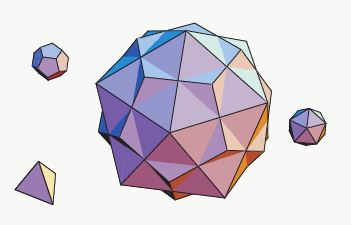
\includegraphics{1.jpg}
\caption{ Poliedros}
\end{center}
\end{minipage}
\end{figure}

\end{document}